\documentclass{article}

\usepackage{fullpage}
\usepackage{color}
\usepackage{amsmath}
\usepackage{url}
\usepackage{verbatim}
\usepackage{graphicx}
\usepackage{parskip}
\usepackage{amssymb}
\usepackage{nicefrac}
\usepackage{listings} % For displaying code
\usepackage{algorithm2e} % pseudo-code

% Answers
\def\ans#1{\par\gre{Answer: #1}}
%\def\ans#1{} % Comment this line to produce document with answers

% Colors
\definecolor{blu}{rgb}{0,0,1}
\def\blu#1{{\color{blu}#1}}
\definecolor{gre}{rgb}{0,.5,0}
\def\gre#1{{\color{gre}#1}}
\definecolor{red}{rgb}{1,0,0}
\def\red#1{{\color{red}#1}}
\def\norm#1{\|#1\|}

% Math
\def\R{\mathbb{R}}
\def\argmax{\mathop{\rm arg\,max}}
\def\argmin{\mathop{\rm arg\,min}}
\newcommand{\mat}[1]{\begin{bmatrix}#1\end{bmatrix}}
\newcommand{\alignStar}[1]{\begin{align*}#1\end{align*}}
\def\half{\frac 1 2}
\def\cond{\; | \;}


% LaTeX
\newcommand{\fig}[2]{\includegraphics[width=#1\textwidth]{a4f/#2}}
\newcommand{\centerfig}[2]{\begin{center}\includegraphics[width=#1\textwidth]{a4f/#2}\end{center}}
\newcommand{\matCode}[1]{\lstinputlisting[language=Matlab]{a4f/#1.m}}
\def\items#1{\begin{itemize}#1\end{itemize}}
\def\enum#1{\begin{enumerate}#1\end{enumerate}}


\begin{document}

\title{CPSC 340 Assignment 4  (due \red{Monday November 14} at 11:55pm)}
\author{}
\date{}
\maketitle
\vspace{-4em}


\blu{Name(s) and Student ID(s):}

\section{Gaussian RBFs and Regularization}

Unfortunately, in practice we often do not know what basis to use. However, if we have enough data then we can make up for this by using a basis that is flexible enough to model any reasonable function. These may perform poorly if we do not have much data, but can perform almost as well as the optimal basis as the size of the dataset grows. In this question you will explore using Gaussian radial basis functions (RBFs), which have this property. These RBFs depend on a parameter $\sigma$, which (like $p$ in the polynomial basis) can be chosen using a validation set. In this question, you will also see how cross-validation allows you to tune parameters of the model on a larger dataset than a strict training/validation split would allow.

\subsection{Regularization}

If you run the demo \emph{example\_RBF.jl}, it will load a dataset and randomly split the training examples into a ``train" and a ``validation" set (it does this randomly since the data is sorted). It will then search for the best value of $\sigma$ for the RBF basis. Once it has the ``best" value of $\sigma$, it re-trains on the entire dataset and reports the training error on the full training set as well as the error on the test set.

A strange behaviour appears: if you run the script more than once it might choose different values of $\sigma$. Sometimes it chooses a large value of $\sigma$ (like $32$) that follows the general trend but misses the oscillations. Other times it sets $\sigma = 1$ or $\sigma=2$, which fits the oscillations better but overfits so achieves a similar test error.\footnote{This behaviour seems to be dependent on your exact setup. Because the $Z^TZ$ matrix with the RBF matrix is really-badly behaved numerically, different floating-point and matrix-operation implementations will handle this in different ways: in some settings it will actually regularizer for you!} \blu{Write a function \emph{leastSquaresRBF}, that fits the model with L2-regularization. Hand in your code, and report the test error you obtain if you train on the full dataset with $\sigma=1$ and $\lambda = 10^{-12}$ (a very small value).}

Hint: to construct an identity matrix in Julia, use the linear algebra package (\emph{using LinearAlgebra}) and then use $I$ to make an identity matrix of the appropriate size (Julia figures out the dimensions for you).

\ans{With best sigma of 1.000, testError = 71.17}
\begin{lstlisting}
using LinearAlgebra
function leastSquaresRBF(X,y,sigma)
	(n,d) = size(X)
	lambda = 10^-12
	Z = rbf(X,X,sigma)
	w = (Z'*Z + lambda*I)\(Z'*y)
	predict(Xhat) = rbf(Xhat,X,sigma)*w
	return LinearModel(predict,w)
end
\end{lstlisting}

\pagebreak


\subsection{Cross-Validation}

Even with regularization, the randomization of the training/validation sets has an effect on the value of $\sigma$ that we choose (on some runs it still chooses a large $\sigma$ value).
This variability would be reduced if we had a larger ``train" and ``validation" set, and one way to simulate this is with \emph{cross-validation}. \blu{\red{Modify the training/validation procedure to use 10-fold cross-validation to select $\sigma$ (with $\lambda$ fixed at $10^{-12}$). Hand in your code and report how this affects the selection of $\sigma$ compared to the original code.}}

\ans{The sigma selected is 1. The selection of this sigma is more stable and relies less on the randomization of the dataset.}
\begin{lstlisting}
shuffledOrder = shuffle(1:n)

include("leastSquares.jl")
minErr = Inf
bestSigma = []
for sigma in 2.0.^(-15:15)
	# Cross validation for 10 folds
	meanError = 0
	folds = 10
	foldSize = Int(n/folds)
	foldInd = 1

	for i in 1:10
		validNdx = shuffledOrder[foldInd:foldInd+foldSize-1]
		trainNdx = setdiff(shuffledOrder,validNdx)
	
		Xtrain = X[trainNdx,:]
		ytrain = y[trainNdx]
		Xvalid = X[validNdx,:]
		yvalid = y[validNdx]
	
		foldInd += foldSize

		# Train on the training set
		model_sigma = leastSquaresRBF(Xtrain,ytrain,sigma)

		# Compute the error on the validation set
		yhat_sigma = model_sigma.predict(Xvalid)
		meanError += sum((yhat_sigma - yvalid).^2)/(n/2)
	end

	meanError /= 10

	@printf("With sigma = %.3f, validError = %.2f\n",sigma,meanError)

	# Keep track of the lowest validation error
	if meanError < minErr
		global minErr = meanError
		global bestSigma = sigma
	end
end
\end{lstlisting}


\pagebreak

\subsection{Cost of Non-Parametric Bases}

When dealing with larger datasets, an important issue is the dependence of the computational cost on the number of training examples $n$ and the number of features $d$.
\blu{
\enum{
\item What is the cost in big-O notation of training a linear regression model with Gaussian RBFs on $n$ training examples with $d$ features (for fixed $\sigma$ and $\lambda$)?
\ans{$O(n^3$}
\item What is the cost of classifying $t$ new examples with this model?
\ans{$O(t^3)$}
\item When is it cheaper to train using Gaussian RBFs than using the original linear basis?
\ans{It is cheaper to train a Gaussian RBF when the number of training examples is lower than the number of features.}
\item When is it cheaper to predict using Gaussian RBFs than using the original linear basis?
\ans{It is cheaper to train a Gaussian RBF when the number of test examples is lower than the number of features.}
}}

\pagebreak

\section{Logistic Regression with Sparse Regularization}

If you run the function \emph{example\_logistic.jl}, it will:
\enum{
\item Load a binary classification dataset containing a training and a validation set.
\item ``Standardize'' the columns of $X$ and add a bias variable.
\item Apply the same transformation to $Xvalidate$.
\item Fit a least squares model, using the sign of $w^Tx_i$ to make predictions.
\item Report the number of features selected by the model (number of non-zero regression weights).
\item Report the error on the training and validation sets.
}
Least squares does ok as a binary classifier on this dataset, but it uses all the features (even though only the prime-numbered features are relevant) and the validation error is above the minimum achievable for this model (which is 1 percent, if you have enough data and know which features are relevant). In this question, you will modify this demo to use the logistic loss and to use different forms of regularization to improve on these aspects.


\subsection{Logistic Regression}

Instead of least squares, modify the script to use logistic regression. You can use the \emph{logReg.jl} file, which implements the training and prediction function for a logistic regresion classifier (using a  version of the \emph{findMin} function that does derivative checking for you and that uses more-clever choices of step-sizes). When you switch to using logistic regression, \blu{report how the following quantities change: the training error, validation error, and number of features}.
\ans{\\
For least squares model: \\
numberOfNonZero = 101 \\ 
trainError = 0.038 \\ 
validError = 0.106 \\
\\
For logistic regression model: \\
numberOfNonZero = 101 \\
trainError = 0.0 \\ 
validError = 0.082 \\
\\
In the values, both the number of features do not change. While the training error for logistics regression decreases to 0, and the validation error also decreases slightly. This might prove to be a better model as such.
}


\subsection{L2-Regularization}

Make a new function, \emph{logRegL2}, that takes an input parameter $\lambda$ and fits a logistic regression model with L2-regularization. Specifically, while \emph{logReg} computes $w$ by minimizing
\[
f(w) = \sum_{i=1}^n \log(1+\exp(-y_iw^Tx_i)),
\]
your new function \emph{logRegL2} should compute $w$ by minimizing
\[
f(w) = \sum_{i=1}^n \left[\log(1+\exp(-y_iw^Tx_i))\right] + \frac{\lambda}{2}\norm{w}^2.
\]
\blu{Hand in the objective function that your updated code minimizes, and using $\lambda=1.0$ report how the following quantities change: the training error, the validation error, the number of features used, and the number of gradient descent iterations.}

\ans{numberOfNonZero = 101 \\
trainError = 0.002 \\ 
validError = 0.074 \\
Iterations = 30 \\
\\
The number of iterations have decreased while the number of non-zeroes stayed the same. The training error is slightly higher, but of an insignificant amount, while the validation error has decreased slightly.
}

\begin{lstlisting}
function logisticObjL2(w,X,y,lambda=1)
	yXw = y.*(X*w)
	f = sum(log.(1 .+ exp.(-yXw))) + lambda/2*sum(w.^2)
	g = -X'*(y./(1 .+ exp.(yXw))) + lambda*w
	return (f,g)
end
\end{lstlisting}




\pagebreak

\subsection{L1-Regularization}

Make a new function, \emph{logRegL1}, that takes an input parameter $\lambda$ and fits a logistic regression model with L1-regularization,
\[
f(w) = \sum_{i=1}^n \left[\log(1+\exp(-y_iw^Tx_i))\right] + \lambda\norm{w}_1.
\]
\blu{Hand in your \emph{logRegL1} code. Using this new code and $\lambda=1$, report the following quantities: the training error, the validation error, and the number of features the model uses.}


You should use the function \emph{findMinL1}, which implements a proximal-gradient method to minimize the sum of a differentiable function $g$ and $\lambda\norm{w}_1$,
\[
f(w) = g(w) + \lambda \norm{w}_1.
\]
 This function has a similar interface to \emph{findMin}, except that you (a) only provide the code to compute the function/gradient of the differentiable part $g$ and (b) need to provide the value $\lambda$.

\ans{numberOfNonZero = 78\\
trainError = 0.008\\
validError = 0.046\\
In this case, the number of features used actually decreased, meaning that more features are now not as important. The training error has increased slightly and the validation error has continuously decreased.
}

\begin{lstlisting}
function logRegL1(X,y,lambda=1)
	(n,d) = size(X)
	
	w = zeros(d,1)
	funObj(w) = logisticObjL1(w,X,y,lambda)

	# Solve least squares problem
	w = findMinL1(funObj,w,lambda)

	# Make linear prediction function
	predict(Xhat) = sign.(Xhat*w)

	# Return model
	return LinearModel(predict,w)
end

function logisticObjL1(w,X,y,lambda=1)
	yXw = y.*(X*w)

	f = sum(log.(1 .+ exp.(-yXw))) + lambda*sum(abs.(w))
	g = -X'*(y./(1 .+ exp.(yXw))) + lambda*sign.(w)
	return (f,g)
end
\end{lstlisting}

\pagebreak

\subsection{L0-Regularization}

The function \emph{logRegL0} contains part of the code needed to implement the \emph{forward selection} algorithm, which approximates the solution with L0-regularization,
\[
f(w) =  \sum_{i=1}^n \left[\log(1+\exp(-y_iw^Tx_i))\right] + \lambda\norm{w}_0.
\]
The `for' loop in this function is missing the part where we fit the model using the subset \emph{Sj}, then compute the score and updates the \emph{minScore/minS}. Modify the `for' loop in this code so that it fits the model using only the features \emph{Sj}, computes the score above using these features, and updates the \emph{minScore/minS} variables (if you want to turn off the diagonistics generated by \emph{findMin}, you can use \emph{verbose = false}).\footnote{Note that Julia doesn't like when you re-define functions, but if you change the variable \emph{Xs} it will actually change the behaviour of the \emph{funObj} that is already defined.}
\blu{Hand in your updated code. Using this new code, set $\lambda = 1$ and report: the training error, the validation error, and the number of features used.}]

Note that the code differs a bit from what we discussed in class, since we assume that the first feature is the bias variable and assume that the bias variable is always included. Also, note that for this particular case using the L0-norm with $\lambda=1$ is equivalent to what is known as the Akaike information criterion (BIC) for variable selection.

\ans{numberOfNonZero = 24\\
trainError = 0.0\\
validError = 0.018\\}

\begin{lstlisting}
# PUT YOUR CODE HERE
w = zeros(length(Sj),1)
w = findMin(funObj,w,verbose=false)
(f,~) = funObj(w)
score = f + lambda*length(Sj)
if score < minScore
	minScore = score
	minS = Sj
end
\end{lstlisting}


\pagebreak

\subsection{L1-Regularization vs. L0-Regularization}

For this problem, the relevant features are the bias variable and the featurs with prime numbers. Given this, \blu{explain how each of the 3 regularizers (L2-regularization, L1-regularization, and L0-regularization) performed in terms of false positives for feature selection (a false positive would be when a feature is selected but it is not relevant). And then explain how each method did in terms of false negatives..}

\ans{For the number of false positives, L2 likely has the most, followed by L1 and then L0. This is as for L2, the number of features chosen is high, and its training error is low while validation error is higher. This proves that the features chosen fits the training dataset more, and thus is liekly for more false positives. The same can be said for L1 regularization compared to L0. \\
\\
For the number of false negatives, it would be harder to determine, however, it is likely that L0 has more false negatives as its number of features chosen is signficantly lower. }
\pagebreak


\section{Multi-Class Logistic}

The function \emph{example\_multiClass} loads a multi-class classification dataset with $y_i \in \{1,2,3,4,5\}$ and fits a `one-vs-all' classification model using binary logistic regression, then reports the validation error and shows a plot of the data/classifier. The performance on the validation set is ok, but could be much better. For example, this classifier never  predicts that examples will be in class 1 (corresponding to the blue circles).

\subsection{Softmax Classification}

Linear classifiers make their decisions by finding the class label $c$ maximizing the quantity $w_c^Tx_i$, so we want to train the model to make $w_{y_i}^Tx_i$ larger than $w_{c'}^Tx_i$ for all the classes $c'$ that are not the true label $y_i$.
Here, $c$ is a possible label and $w_{c'}$ is \textbf{row} $c'$ of $W$. Similarly, $y_i$ is the training label, $w_{y_i}$ is \textbf{row} $y_i$ of $W$, and in this setting we are assuming a discrete label $y_i \in \{1,2,\dots,k\}$. Before we move on to implementing the softmax classifier to fix the issues raised in the introduction, let's do a simple example:

Consider the dataset below, which has $30$ training examples, $2$ features, and $3$ class labels:\\
\begin{center}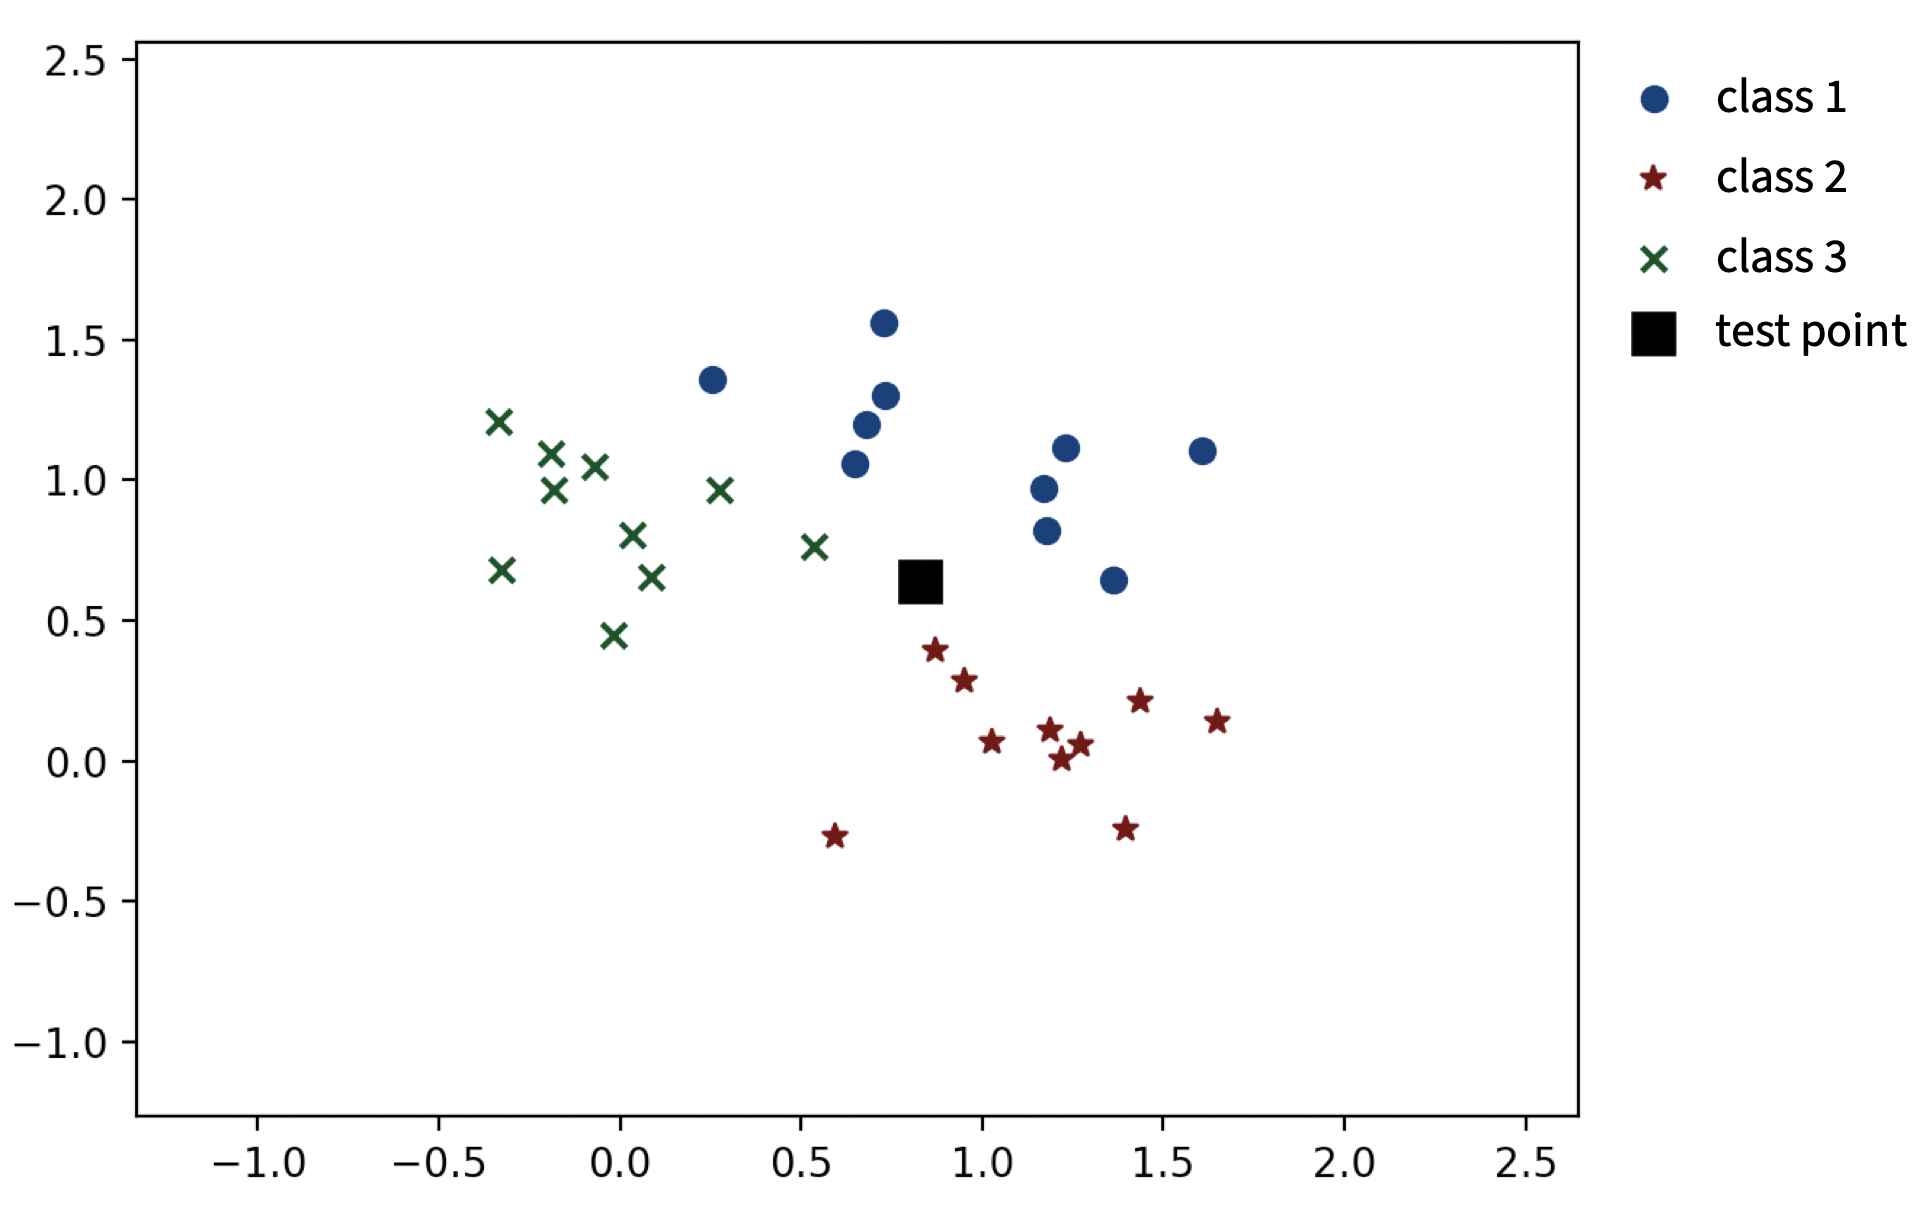
\includegraphics[scale=0.3]{a4f/softmaxData.png}\end{center}
Suppose that we want to classify the black square at the location
\[
\hat{x} = \begin{bmatrix}+0.84 \\ +0.64\\ \end{bmatrix}.
\]
Suppose that we fit a multi-class linear classifier including bias variable using the softmax loss, and we obtain the following weight matrix:
\[
W =
\begin{bmatrix}
+1.62 & +3.47 & +0.00\\
-3.83 & +0.67 & +4.90\\
+2.22 & -4.13 & +3.37\\
\end{bmatrix}.
\]
\blu{
\begin{enumerate}
\item What is the meaning of the rows $w_i$ in the matrix $W$?
\ans{The row $w_i$ represents the weight of the logistic regression for the class label of i.}
\item Under this model, what class label would we assign to the test example? (show your work)
\ans{$P(y = 1 | x) = 1.62 + 3.47*0.84 = 4.5348 \\
P(y = 2 | x) = -3.83 + 0.67*0.84 + 4.9*0.64 = -0.1312 \\
P(y = 3 | x) = 2.22 + -4.13 * 0.84 + 3.37 * 0.64 = 0.9076$\\
x has the highest probability to be in class 1, and should be classified as class 1.}
\end{enumerate}}



\pagebreak

\subsection{Softmax Loss}

Using a one-vs-all classifier hurts performance because the classifiers are fit independently, so there is no attempt to calibrate the \textbf{rows} of the matrix $W$. An alternative to this independent model is to use the softmax loss function, which for $n$ training examples is given by
\[
f(W) = \sum_{i=1}^n \left[-w_{y_i}^Tx_i + \log\left(\sum_{c' = 1}^k \exp(w_{c'}^Tx_i)\right)\right].
\]
\blu{Derive the partial derivative $\frac{\partial f}{\partial W_{jc}}$ of this loss function with respect to a particular element $W_{cj}$ (the variable in row $c$ and column $j$ of the matrix $W$)}. Try to simplify the derivative as much as possible (but you can express the result in summation notation).

Hint: for the gradient you can use $x_{ij}$ to refer to element $j$ of example $i$. For the first term you will need to separately think about the cases where $c=y_i$ and the cases where $c\neq y_i$. You may find it helpful to use an `indicator' function, $I(y_i = c)$, which is $1$ when $y_i = c$ and is $0$ otherwise. Note that you can use the definition of the softmax probability to simplify the second term of the derivative.


\pagebreak

\subsection{Softmax Classifier}

Make a new function, \emph{softmaxClassifier}, which fits $W$ using the softmax loss from the previous section  instead of fitting $k$ independent classifiers. \blu{Hand in the code and report the validation error}.

Hint: you will want to use the \emph{derivativeCheck} option in \emph{findMin.jl} to check that your gradient code is correct. Also, note that \emph{findMin.jl} expects that the parameter vector and gradient are \emph{column vectors}. The easiest way to work around these issues is to use the \emph{reshape} command: call \emph{findMin.jl} with a $dk \times 1$ vector $w$ and at the start of your objective function, reshape $w$ to be a $k \times d$ matrix $W$, then compute the $k \times d$ matrix of partial derivatives, and finally reshape this to be the $dk \times 1$ gradient vector.

\pagebreak

\subsection{Cost of Multinomial Logistic Regression}

Assuming that we have
\items{
\item $n$ training examples.
\item $d$ features.
\item $k$ classes.
\item $t$ testing examples.
\item $T$ iterations of gradient descent for training.
}
\blu{\enum{
\item In big-$\mathcal{O}$ notation, what is the cost of training the softmax classifier?
\ans{}
\item In big-$\mathcal{O}$ notation, what is the cost of classifying the test examples?
\ans{}
}}

\pagebreak

\section{Very-Short Answer Questions}

\enum{
\item If we fit a linear regression model and then remove all features whose associated weight is small, why is this an ineffective way of performing feature selection?
\ans{This may be due to the magnitude or weight of the features. For instance, if one was in the units of kilometers, while another is in the units of grams, it would not be fair to remove the smaller weight as kilometers is in a bigger unit.}
\item Given $3$ features $\{f_1, f_2, f_3\}$, provide an argument that illustrates why the forward selection algorithm is not guaranteed to find an optimal subset of features.
\ans{In the case where there may be some correlation between 2 features. For instance, if there is taco and tuesday, if forward selection selects "tuesday" before "taco", it will consider that "tuesday" is the determining feature for stomachache, while in reality, taco is the determining cause.}
\item What is a setting where you would use the L1-loss, and what is a setting where you would use L1-regularization?
\item Among L0-regularization, L1-regularization, and L2-regularization: which yield convex objectives? Which yield unique solutions? Which yield sparse solutions?
\ans{The L1-regularization and L2-regularization both yield convex objectives. This is as they both use norms, which are convex in nature. L0 would not produce the same convexity as it considers the number of non-zero feature weights. \\
The L2-regularization will yield unique solutions, while L0 and L1 may not. \\
L0 and L1 regularization both yield sparse solutions, while the L2 may not.
}
\item What is the effect of $\lambda$ in L1-regularization on the sparsity level of the solution? What is the effect of $\lambda$ on the two parts of the fundamental trade-off?
\ans{As $\lambda$ increase for L1, the sparsity level of the solution increases. As such, training error tends to increase while the test error would decrease.}
\item Suppose you have a feature selection method that tends not generate false positives but has many false negatives (it misses relevant variables). Describe an ensemble method for feature selection that could improve the performance of this method.
\ans{}
\item How does the hyper-parameter $\sigma$ affect the shape of the Gaussian RBFs bumps? How does it affect the fundamental tradeoff?
\ans{The hyper-parameter $\sigma$ changes the bumps of the Gaussian RBF. As $\sigma$ increases, the bumps width increases. \\
As $\sigma$ increases, the training error goes up, but the validation error goes down.}
\item What is the main problem with using least squares to fit a linear model for binary classification?
\ans{For a binary classification, fitting a linear model may cause for the linear model to average out for the lowest squared error. For instance in the case of number of "vicodin" appearances, for the mail to be spam, the number of times can be infinitely many, while for not-spam, it is limited. Thus the model does not fit accurately due to averaging.}
\item Suppose a binary classification dataset has 3 features. If this dataset is ``linearly separable'', what does this precisely mean in three-dimensional space?
\item Why do we not minimize $\max(0, -y_i w^\top x_i)$ when we fit a binary linear classifier, even though it’s a convex approximation to the 0-1 loss?
\item For a linearly-separable binary classification problem, how does an SVM classifier differ from a classifier found using the perceptron algorithm?
\item Which of the following methods produce linear classifiers? (a) binary least squares as in Question 3, (b) the perceptron algorithm, (c) SVMs, (d) logistic regression, and (e) KNN with $k=1$ and $n=2$.
\item Why do we use the polynomial kernel to implement the polynomial basis when $d$ and $p$ (degree of polynomial) are large?
\item What is the relationship between the softmax loss and the softmax function?
}

\pagebreak

\section*{Project Proposal (OPTIONAL FOR 340 STUDENTS)}

For 532M students, there is a project component to the course that will be worth 20\% of your final grade. For 340 students, there is no requirement to do a project. However, 340 students have the option to do a project anyway for the possibility of obtaining a higher grade: your project grade can replace either your 2 lowest assignment scores or your midterm score (whicheve helps you more).\footnote{The course is \emph{not} graded on a curve, so 340 students are not hurt by choosing the to skip the project.}

These projects are done in \blu{groups of 2-3}. The final deliverable will be a \blu{6-page report that is due near the end of the exam period} (something like December 22nd, minus a few days so we have time to grade). It is expected that this project will be a literature survey, but research projects are also ok.

There aren't really any restrictions on the group compositions: 340 students can work with 532M students, auditors can work with registered students, and you can combine this project with a project from another one of your classes (assuming you get the other instructor's permission, and even if not all students in the other class are registered in this class). The only combinations I really want to avoid are having students do projects with the TAs (due to the obvious conflict of interest), project groups that have no students enrolled in 340 or 532M, or projects that contain people taking no CPSC classes.

If you are in 532M, or in 340 and want to do a project, for the final part of this assignment you must a \blu{submit a project proposal} for your course project. The proposal should be a maximum of 2 pages (and 1 page or half of a page is ok if you can describe your plan concisely). The proposal should be written for the instructors and the TAs, so you don't need to introduce any ML background but you will need to introduce non-ML topics.

\blu{You should submit this question as a group on Gradescope, separate from the other assignment questions.}

There is quite a bit of flexibility in terms of the type of project you do, as I believe there are many ways that people can make valuable contributions to research. However, note that ultimately the final deliverable for the project will be a report that emphasizes a particular ``contribution" (i.e., what doing the project has added to the world).
The reason for this, even though it's strange for some possible projects, is that this is the standard way that results are communicated to the research community.

\blu{The three mains ingredients of the project proposal are:
\begin{enumerate}
\item What problem you are focusing on.
\item What you plan to do.
\item What will be the ``contribution".
\end{enumerate}
}
Also, for the course project note that negative results (i.e., we tried something that we thought would work in a particular setting but it didn't work) are acceptable (and often unavoidable).

I encourage you to follow the following default ``template'' for the project:
\enum{
\item \textbf{Literature review}: you pick a specific topic in ML, read at least 10 papers on the topic, then write a report summarizing what has been done on the topic and what are the most promising directions of future work. In this case, the contribution would be your summary of the relationships between the existing works, and your insights about where the field is going.
}
The advantage of the above template is that the project will take a somewhat-predictable amount of time. If you want to explore a different style of project, here are some standard ``templates'':
\enum{
\setcounter{enumi}{1}
\item \textbf{Application bake-off}: you pick a specific application (from your research, personal interests, or maybe from Kaggle) or a small number of related applications, and try out a bunch of techniques (e.g., random forests vs. logistic regression vs. generative models). In this case, the contribution would be showing that some methods work better than others for this specific application (or your contribution could be that everything works equally well/badly).
\item \textbf{New application}: you pick an application where people aren't using ML, and you test out whether ML methods are effective for the task. In this case, the contribution would be knowing whether ML is suitable for the task.
\item \textbf{Scaling up}: you pick a specific machine learning technique, and you try to figure out how to make it run faster or on larger datasets. In this case, the contribution would be the new technique and an evaluation of its performance, or could be a comparison of different ways to address the problem.
\item \textbf{Improving performance}: you pick a specific machine learning technique, and try to extend it in some way to improve its performance. In this case, the contribution would be the new technique and an evaluation of its performance.
\item \textbf{Generalization to new setting}: you pick a specific machine learning technique, and try to extend it to a new setting (for example, making a multi-label version of random forests).  In this case, the contribution would be the new technique and an evaluation of its performance, or could be a comparison of different ways to address the problem.
\item \textbf{Coding project}: you pick a specific method or set of methods, and build an implementation of them. In this case, the contribution could be the implementation itself or a comparison of different ways to solve the problem.
\item \textbf{Theory}: you pick a theoretical topic (like the variance of cross-validation), read what has been done about it, and try to prove a new result (usually by relaxing existing assumptions or adding new assumptions). The contribution could be a new analysis of an existing method, or why some approaches to analyzing the method will not work.
\item \textbf{Reproduction}: you take a recent paper published in one of the top machine learning venue (either NeurIPS, ICML, ICLR, AI/Stats, or JMLR), and try to reproduce the results in the paper.
}
The above are just suggestions, and  projects could mix several of these templates together, but if you are having trouble getting going then it's best to stick with one of the above templates (and again I recommend doing the literature review). Also note that the project can focus on topics not covered in the course (like GANs), so there is flexibility in the topic, but the topic should be closely-related to ML.

\blu{This question is mandatory but will not be formally marked: it is just a sanity check that you have at least one project idea that has an appropriate topic and scope, that you find a group early, and that you  allocate some time to thinking about the project.}
Also, there is flexibility in the choice of project topics even after the proposal: if you want to explore different topics you can ultimately choose to do a project that is unrelated to the one in your proposal (and changing groups is ok too). If you aren't sure what to do, go bug the TAs in office hours (which is a good idea even if you are sure what you want to).
\end{document}
